\section{Opis Modelu SI}\label{sec:opis-modelu-si}

Model sztucznej inteligencji został zaprojektowany w celu klasyfikacji zdjęć kości ośmiościennych k8 do jednej z ośmiu klas,
odpowiadających cyfrom od 1 do 8 na każdej ze ścianek.
Do implementacji modelu wykorzystano przede wszystkim moduł TensorFlow~\cite{tensorflow_docs}
oraz wchodzący obecnie w jego skład Keras~\cite{keras_docs},
który umożliwia łatwe tworzenie i trenowanie sieci neuronowych.


%% uselesss :(( \textit{Biblioteka Keras jest wygodnym opakowaniem (wrapperem) dla modeli DL używanych do oszacowań klasyfikacji lub regresji]} [Donald J. Norris, 2020 s. 355 wydanie APN PROMISE SA]


\subsection{Przygotowanie danych}\label{subsec:przygotowanie-danych}

Dane wejściowe zostały podzielone na zestawy treningowy i walidacyjny w proporcji 70:30.
W celu zwiększenia różnorodności danych treningowych zastosowano techniki augmentacji obrazów dostępne w klasie
\texttt{ImageDataGenerator}~\cite{keras_imagedatagenerator}, takie jak:

-- TODO -- zakresy zmienności zoom, shear itd
\begin{itemize}
    \item obrót o losowy kąt w zakresie do 90°,
    \item przesunięcia poziome i pionowe,
    \item transformacje perspektywiczne (ang. shear),
    \item losowe przybliżenia lub oddalenia (ang. zoom).
\end{itemize}

Wszystkie augmentacje przedstawiono na rysunkach~\ref{fig:5augment}
Dodatkowo, obrazy są normalizowane do zakresu $[0, 1]$, co pozwala na skuteczniejsze działanie sieci neuronowej.


\begin{figure}[h]
    \centering
    \begin{subfigure}[t]{0.32\linewidth}
        \centering
        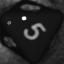
\includegraphics[width=\linewidth]{chapters/04-czytanie/figures/5_preprocessed}
        \caption{Obraz po preprocessingu, bazowy dla augmentacji.}
        \label{fig:5raw}
    \end{subfigure}
    \hfill
    \begin{subfigure}[t]{0.32\linewidth}
        \centering
        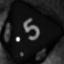
\includegraphics[width=\linewidth]{chapters/04-czytanie/figures/5_rotate}
        \caption{Obraz po obrocie.}
        \label{fig:5rotate}
    \end{subfigure}
    \hfill
    \begin{subfigure}[t]{0.32\linewidth}
        \centering
        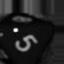
\includegraphics[width=\linewidth]{chapters/04-czytanie/figures/5_shift}
        \caption{Obraz po przesunięciu.}
        \label{fig:5move}
    \end{subfigure}

    \vspace{0.5cm} % Odstęp między wierszami obrazków

    \begin{subfigure}[t]{0.32\linewidth}
        \centering
        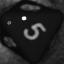
\includegraphics[width=\linewidth]{chapters/04-czytanie/figures/5_shear}
        \caption{Obraz po ścinaniu.}
        \label{fig:5shear}
    \end{subfigure}
    \hfill
    \begin{subfigure}[t]{0.32\linewidth}
        \centering
        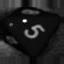
\includegraphics[width=\linewidth]{chapters/04-czytanie/figures/5_zoom}
        \caption{Obraz po powiększeniu.}
        \label{fig:5zoom}
    \end{subfigure}
    \hfill
    \begin{subfigure}[t]{0.32\linewidth}
        \centering
        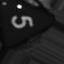
\includegraphics[width=\linewidth]{chapters/04-czytanie/figures/combined_1}
        \caption{Obraz wynikowy.}
        \label{fig:5combined}
    \end{subfigure}

    \caption{Różne składowe augmentacji obrazów uczących}
    \label{fig:5augment}
\end{figure}


W szczególności należy zaznaczyć, że finalnie uniknięto początkowo przeoczonego błędu,
jakim jest tworzenie obrazów lustrzanych w wyżej wymienionych transformacjach, gdyż obrazy lustrzane
sprawiały, że ścianki 2 oraz 5 były znacznie gorzej rozróżnialne przez wytrenowany model.
Problem nie był początkowo łatwy do wykrycia, gdyż zdjęcia odbite zarówno w pionowej jak i poziomej osi były poprawne,
a niepoprawne były te odbite tylko wobec jednej osi, czego przykład można zaobserwować na rysunku~\ref{fig:25confusion}.


\begin{figure}[h]
    \centering
    \begin{subfigure}[t]{0.45\linewidth}
        \centering
        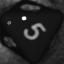
\includegraphics[width=\linewidth]{chapters/04-czytanie/figures/5_preprocessed}
        \caption{Zdjęcie przedstawiające 5}
        \label{fig:5_confusion}
    \end{subfigure}
    \hfill
    \begin{subfigure}[t]{0.45\linewidth}
        \centering
        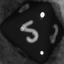
\includegraphics[width=\linewidth]{chapters/04-czytanie/figures/2_mirror}
        \caption{Zdjęcie przedstawiające 2, odbite lustrzanie}
        \label{fig:2_confusion}
    \end{subfigure}
    \caption{Nieczytelne ujęcia wynikające z dłuższego niż przewidywany ruchu kości}
    \label{fig:25confusion}
\end{figure}

\subsection{Architektura modelu}\label{subsec:architektura-modelu}

\subsection{Użyte funkcje aktywacji i rodzaje warstw}\label{subsec:uzyte-funkcje-aktywacji-i-rodzaje-warstw}

\subsubsection{Sieci splotowe (CNN)}
Sieci splotowe to rodzaj sieci neuronowych, które szczególnie dobrze sprawdzają się w zadaniach związanych
z przetwarzaniem obrazów, takich jak rozpoznawanie obiektów, klasyfikacja czy segmentacja.
Główna różnica między siecią splotową a tradycyjną siecią neuronową polega na tym,
że w sieciach splotowych stosuje się operację splotu, która umożliwia wydobycie lokalnych cech z obrazu,
redukując liczbę parametrów i umożliwiając efektywniejsze uczenie się reprezentacji obrazu. \\
Warstwy splotowe w sieci CNN wykonują operację splotu, polegającą na zastosowaniu filtrów (jąder) na obrazie wejściowym,
co pozwala na wyodrębnienie różnych cech (np. krawędzi, tekstur) w różnych lokalizacjach obrazu.
Kolejne warstwy splotowe uczą się coraz bardziej złożonych cech w miarę postępującej abstrakcji,
dzięki czemu sieć może rozpoznać skomplikowane wzorce w danych wejściowych.

\subsubsection{Warstwa gęsta (Dense)}
Warstwa gęsta (ang. Dense, fully connected layer), to warstwa w której każdy neuron jest połączony z każdym neuronem w poprzedniej warstwie.
Tego typu warstwy zwykle znajdują się na końcu sieci, po warstwach splotowych, i służą do agregowania informacji uzyskanych
z wcześniejszych warstw w celu podjęcia ostatecznej decyzji, jak w klasyfikacji.
W przypadku tego modelu, warstwy gęste przekształcają dane wyjściowe z warstw splotowych w wektory,
które reprezentują cechy odpowiednie do klasyfikacji.


Użyte funkcje aktywacji:
%o, sprawdziłem nawet, to NIE JEST to co mi chat geenrował, bo mi się nie podobało i przepisywałem XD
% zupełnie zapomniałem o tym XDD
\begin{itemize}
    \item ReLU -- najczęściej stosowana funkcja aktywacji w sieciach splotowych.
    Jest to funkcja, która zwraca 0 dla wszystkich ujemnych wartości i zachowuje wartość dodatnią dla wszystkich liczb dodatnich.
    ReLU pozwala na szybkie i efektywne uczenie się sieci, eliminując problem zanikania gradientu,
    który występuje w tradycyjnych funkcjach aktywacji, takich jak sigmoidalna.
    \item Softmax -- to funkcja aktywacji, która jest używana w zadaniach klasyfikacyjnych,
    szczególnie w przypadku, gdy mamy do czynienia z wieloma klasami.
    Softmax przekształca wyjścia z warstwy gęstej w rozkład prawdopodobieństwa,
    gdzie suma prawdopodobieństw dla wszystkich klas wynosi 1.
\end{itemize}

\subsection{Budowa sieci neuronowej}\label{subsec:budowa-sieci-neuronowej}
Model jest wielowarstwową siecią splotową (ang. convolutional neural network, CNN),
składającą się z następujących elementów:

\begin{enumerate}
    \item Warstwa wejściowa o rozmiarze 64x64 pikseli i jednym kanale (skala szarości),
    \item Trzech warstw splotowych z funkcją aktywacji ReLU oraz warstw max poolingu:
    \begin{enumerate}
        \item Pierwsza warstwa splotowa z 32 filtrami o rozmiarze 3x3,
        \item Warstwa max poolingu z jądrem 2x2,
        \item Druga warstwa splotowa z 64 filtrami o rozmiarze 3x3,
        \item Warstwa max poolingu z jądrem 2x2,
        \item Trzecia warstwa splotowa z 128 filtrami o rozmiarze 3x3,
        \item Warstwa max poolingu z jądrem 2x2,
    \end{enumerate}
    \item Warstwa spłaszczająca (Flatten),
    \item Dwóch w pełni połączonych warstw (Dense):
    \begin{enumerate}
        \item Pierwsza warstwa Dense z 128 neuronami i funkcją aktywacji ReLU,
        \item Druga warstwa Dense z 8 neuronami i funkcją aktywacji softmax, przeznaczona do klasyfikacji na 8 klas.
    \end{enumerate}
\end{enumerate}

W przypadku zmiany kości na taką z inną liczbą ścianek, np.
na również rozważane w fazie koncepcyjnej kości czworościenną, sześciościenną, albo szesnastościenną,
ostatnia warstwa musiałaby również ulec odpowiedniej zmianie,
tak aby liczba neuronów odpowiadała liczbie ścianek na używanej kości.

\subsection{Trenowanie modelu}\label{subsec:trenowanie-modelu}

Model został nauczony z wykorzystaniem optymalizatora Adam~\cite{kingma2014adam, keras_adam},
funkcji straty entropii krzyżowej~\cite{crossentropy} dostępnej w module tensorflow jako sparse categorical crossentropy~\cite{tensorflow_loss},
oraz metryki dokładności (ang. accuracy)~\cite{tensorflow_accuracy}.
Proces trenowania obejmował dobraną eksperymentalnie liczbę 20 epok, gdyż dalsze zwiększanie liczby epok nie przynosiło istotnej poprawy wydajności zwiększając jedynie czas obliczeń.
Na wejściu, model oczekiwał obrazu przedstawiającego górną ściankę kości, przekształconego odpowiednio, a więc tak jak opisano w~\ref{sec:preprocessing}.


\subsection{Wyniki}\label{subsec:wyniki}

Podczas trenowania osiągnięto następujące końcowe wyniki:

\begin{itemize}
    \item Dokładność na zbiorze treningowym: 0,9375
    \item Dokładność na zbiorze walidacyjnym: 1,0
    \item Strata na zbiorze treningowym: 0,0786
    \item Strata na zbiorze walidacyjnym: 0,0274
\end{itemize}

Wyniki zostały również zwizualizowane na wykresach (rysunki~\ref{fig:ModelAcc} oraz~\ref{fig:ModelLoss})
przedstawiających zmianę dokładności i straty w trakcie trenowania.

\begin{figure}[H]
    \centering
    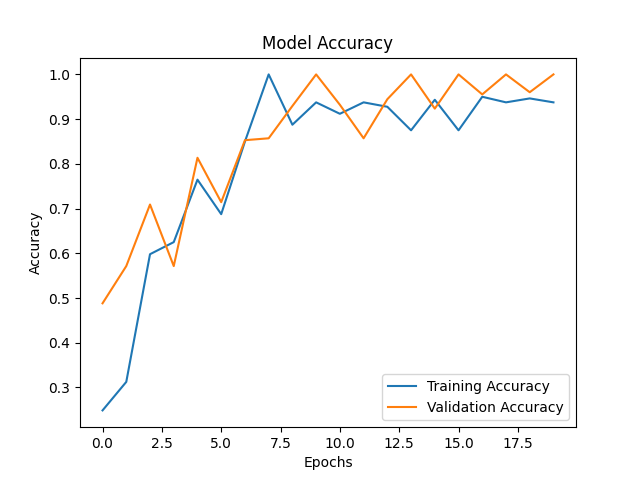
\includegraphics[width=0.7\textwidth]{chapters/04-czytanie/figures/ModelAcc1}
    \caption{Wykres dokładności modelu.}
    \label{fig:ModelAcc}
\end{figure}

\begin{figure}[H]
    \centering
    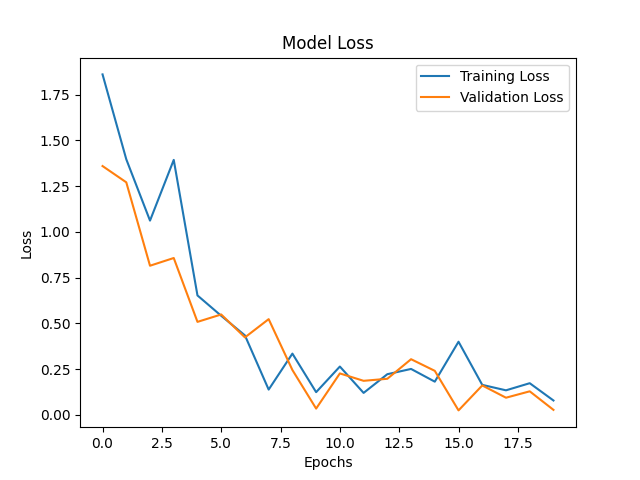
\includegraphics[width=0.7\textwidth]{chapters/04-czytanie/figures/ModelLoss1}
    \caption{Wykres straty modelu.}
    \label{fig:ModelLoss}
\end{figure}

Model został zapisany w formacie \texttt{.keras} i jest gotowy do użycia w systemie rozpoznawania liczb na ośmiościennej kości,
opisanym w kolejnej sekcji.
